\documentclass{article}
\usepackage{graphicx} % Required for inserting images

\title{Branched optimal transport}
\author{Antonio De Rosa, Dario Filatrella, Aida Khajavirad}
\date{August 2024}

% Packages
\usepackage{amsmath}
\usepackage{tikz-cd}
\usepackage{amsfonts}
\usepackage{amsthm}
\usepackage{amssymb}

% Document

\renewcommand\qedsymbol{$\cdot$}


\begin{document}

    \maketitle



    \section{Relation between Euclidean Steiner Tree and MMX}

\subsection{Euclidean Steiner Tree}

Given a set of points $P$ in $\mathbb{R}^N$, the Euclidean Steiner Tree problem is to find the shortest tree (possibly
adding new points) that connects all points in $P$. Calling the resulting graph $G = (V, E)$, the cost of the tree is
\begin{equation}
    \sum_{(u, v) \in E} \|u - v\|
\end{equation}
Where $\| \cdot \|$ is the Euclidean norm.

\subsection{MMX}
The MMX is defined in \ref{Paper linkato} as follows: given a set of points $P$ in $\mathcal{R}^N$, the minimization problem is:

\begin{align}
    \text{(MMX)}: \; \min &\sum_{[i,j] \in E_1} \|a^i - x^j\| y_{ij} + \sum_{[i,j] \in E_2} \|x^i - x^j\| y_{ij}, \\
    & \sum_{j \in S} y_{ij} = 1 \quad \text{for } i \in P, \\
    & \sum_{i \in P} y_{ij} + \sum_{k < j, k \in S} y_{kj} + \sum_{k > j, k \in S} y_{jk} = 3 \quad \text{for } j \in S, \label{MMX:connectivity_steiner} \\
    & \sum_{k < j, k \in S} y_{kj} = 1 \quad \text{for } j \in S - \{p+1\},  \\
    & y_{ij} \in \{0, 1\}, \quad [i, j] \in E, \quad x^i \in \mathbb{R}^n, \quad i \in S.
\end{align}

Where: \begin{itemize}
           \item $P$ is the set of terminals,
           \item $S$ is the set of Steiner points (in this case $S = \{|P| + 1, ..., 2|P|-2\}$),
           \item $E_1$ is the set of edges connecting terminals to Steiner points,
           \item $E_2$ is the set of edges connecting Steiner points
\end{itemize}

\subsection{Relation between the two problems}

The MMX problem "solves" the ESTP in the sense that under certain conditions, the optimal solution of MMX corresponds to
the optimal EST.
Explicitly, we can construct a function $\phi$ that maps feasible solutions of MMX to feasible solutions of ESTP and such
that the following commutative diagram holds:

\[
    \begin{tikzcd}
        & \mathbb{R}  \\
        MMX \arrow[ur, "Obj"] \arrow[rr, "\phi"'] & & EST  \arrow[ul, "Obj"]
    \end{tikzcd}
\]

Where $Obj$ is the objective function of the respective problems and MMX and EST are the feasible regions.

\subsection{Definition of $\phi$}
The function $\phi$ maps $\mathbb{R}^{N (|P|-2)} \times \{0,1\}^{|E|}$ to a graph in $\mathbb{R}^N$ as follows:

\begin{enumerate}
    \item For each $i \in P$, add a terminal at $a^i$.
    \item For each $j \in S$, add a vertex $v_j$ at $x^j$.
    \item For each $[i,j] \in E$ with $y_{ij} = 1$, add an edge between $v_i$ and $v_j$.
\end{enumerate}

There are a few issues with this identification: $\phi$ is neither injective (there is a permutation invariance in the index of both
Steiner points and terminals) nor surjective, as for instance, the number of vertices is fixed. It is known \ref{Boh} that the number of Steiner points
in an optimal EST cannot be bigger than the ones included in MMX, but it could be lower (in the paper it is specified that
this formulation only holds for full Steiner topologies).
It is easy to see that the objective functions are the same as they both sum the Euclidean distances of the active edges.


\textbf{Claim} Calling MMX and EST the respective feasible regions, we have that $\phi(MMX) \subseteq EST$.

\begin{proof}
    Let $x \in MMX$ and $G = \phi(x)$. We need to show that $G$ is a tree (so connected and loop-free).
    By the first constraints, we know each terminal is connected to a Steiner point and constraint (\ref{MMX:connectivity_steiner}) ensures that
    all Steiner points are connected, so $G$ is connected.
    By edge counting, we deduce that $G$ is a tree.
\end{proof}



\textbf{Claim} The optimal solution of MMX is also optimal for ESTP.

\begin{proof}
    We know from \ref{Libro di optimal transport} that the optimal solution for the ESTP is a tree with
    number of vertices $|V| \le 2|P| - 2$ and degree of each vertex $d(v) \le 3$.
    We can show that for each graph with those properties there is an element in $MMX$ that maps to it.
    In $MMX$ the degree of terminals is fixed to 1 but we can add a Steiner point with coordinates equal to the terminal
    (so allowing a degenerate solution) and make the following construction (for the case $d(v) = 2$):

    OLD PART:
    We add a vertex $i$ with coordinate $x_i = a_j$, we activate edge (of length 0) connecting $i$ to $j$. Then the two
    edges connecting $j$ to the other points are attached to $i$, in this way the degree of the degenerate Steiner point is
    3 and the degree of the terminal is 1.
    We can do a similar construction (but with 2 Steiner points) for the case $d(v) = 3$.
    We still need to do some edges and vertices counting to finish the proof (maybe an induction on the number of vertices?).

    NEW PART:
    We will not do an induction but provide a procedure to add Steiner points until there are enough of them, while keeping
    the graph structure the same. We will then show that those operation preserve all the properties of the MMX problem.

    By doing some edge counting we know that
    \begin{equation}
        |E| = \frac{1}{2} \left( 3|S| + \sum_{i \in P} d(i) \right)
    \end{equation}
    Which implies that:
    \begin{equation}
        \sum_{i \in P} d(i) = 2|P| - 2 - |S|
    \end{equation}
    If $|S| = 2|P| - 2$ we are done, otherwise we can find a terminal $i$ with $d(i) = 2,3$ and add 1 or 2 Steiner points respectively.
    \begin{itemize}

        \item Case $d(i) = 1 $: we add a Steiner point $s$ with connection to the two points connected to $i$ and remove the edge
        connecting $i$ to the other terminal. We also connect $s$ to the terminal $i$.

        \item Case $d(i) = 2$: Calling the points connected to $i$ $z_1, z_2, z_3$ we add two Steiner points $s_1, s_2$ and connect
        $s_1$ to $(z_1, s_2, i)$ and $s_2$ to $(s_1, z_2, z_3)$.
    \end{itemize}

    In this way we preserve connectedness, loop-freeness and the number of (non-degenerate) vertices. Connectedness implies
    \ref{MMX:connectivity_steiner} up to reordering of the Steiner points.
    We can repeat the procedure until $|S| = |P| - 2$ which is our desired number of Steiner points.
    We get that the degree of every terminal is 1 and the degree of every Steiner point is 3, so all the conditions
    of MMX are satisfied.


\end{proof}


\section{Relation between Euclidean Steiner Tree and branched transport}

\subsection{Definition of branched transport}
For now, I will use the Lagrangian formulation of branched transport, as defined in \ref{Libro di branched transport}.

Given $X \subset \mathbb{R}^N$ compact and two measures of equal mass $\mu^+$ and $\mu^-$ on $X$, a traffic plan is
a measure $P$ on $K$ that transports $\mu^+$ to $\mu^-$.
Formally, consider the maps $\pi_0, \pi_\infty : K \rightarrow X$ given by $\pi_0(\gamma) = \gamma(0)$ and $\pi_\infty(\gamma) = \gamma(T(\gamma))$,
$P$ is a traffic plan if:
\[
    \mu^+ = (\pi_0)_{\#}P, \quad \mu^- = (\pi_\infty)_{\#}P
\]

\subsection{Parameterized Traffic Plans}
The next paragraph is copied from the book:


According to Skorokhod theorem (Theorem A.3 p. 185), we can parameterize any traffic plan $P$ by a measurable function
$\chi : \Omega = [0, |\Omega|] \rightarrow K$ such that $P = \chi_{\#} \lambda$, where $\lambda$ is the Lebesgue measure
on $[0, |\Omega|]$. We shall set $\chi(\omega, t) := \chi(\omega)(t)$ and consider it as a function of the variable pair
$(\omega, t)$.

With this formulation the energy (or cost) of a parametrized traffic plan is:
\begin{equation}
    E^{\alpha}(P) = \int_{\mathbb{R}^N} |x|_P^{\alpha} d \mathcal{H}^1(x)
\end{equation}
There are also other formulations and under some assumptions they are equivalent. In particular there should be no problem
for finite atomic measures.

\subsection{Relation between branched transport and ESTP}

We can reduce any ESTP (in the algorithmic sense) to an instance of a branched transport problem.
Given a set of terminals $P = \{a^1, ..., a^{|P|}\}$ we can define:
\begin{equation}
    \mu^+ = \delta_{a^1} \quad \mu^- = \frac{1}{|P| - 1}\sum_{i = 2}^{|P|} \delta_{a^i}
\end{equation}
and set $\alpha =0$ in the cost function.
We can then use results from branched transport to say that the optimal parametrized
traffic plan is a graph and it is loop-free. We will now prove that it is connected and conclude that it is a tree.

For each terminal $a^i$ (with $i>1$) we have a subset $A_i \subset [0,1]$ such that $\chi(A_i)$ are all paths terminating at $a^i$ and
$\chi(A_i)(0) = a_1$.
We can easily conclude that every terminal is connected to $a_1$ and therefore the graph is connected.




    \section{Generalization of MMX}

    \subsection{Things to do}
    \begin{itemize}
        \item Write down formulation for alpha different from 0
        \item Show it is correct
        \item Add degree constraint
        \item Run computations for the degree
        \item Look into the other optimization to see if the closest points rule is also ok
        \item Use theoretical results for LB improvement (Wesserstein distance)
    \end{itemize}

    \begin{align}
        \text{(MMX)}: \; \min &\sum_{[i,j] \in E_1} (f^{\alpha}_{ij} + f^{\alpha}_{ji})\|a^i - x^j\| y_{ij} + \sum_{[i,j] \in E_2} (f^{\alpha}_{ij} + f^{\alpha}_{ji})\|x^i - x^j\| y_{ij} \\
        & \sum_{j \in S} y_{ij} = 1 \quad \text{for } i \in P, \\
        & \sum_{k < j, k \in S} y_{kj} = 1 \quad \text{for } j \in S - \{p+1\},  \\
        & \sum_{i \in S \cup P} f_{ij} - \sum_{i \in S \cup P} f_{ji} = m_j \quad \text{for } j \in P, \\
        & \sum_{i \in S \cup P} f_{ij} - \sum_{i \in S \cup P} f_{ji} = 0 \quad \text{for } j \in S, \\
        & f_{ij} \le y_{ij} \quad \text{for } i,j \in S \cup P \\
        & y_{ij} \in \{0, 1\}, \quad [i, j] \in E, \quad x^i \in \mathbb{R}^n, \quad i \in S. \\
        & y_{ij} = y_{ji} \quad \text{for } i,j \in S \cup P \\
        & f_{ij} \in [0,1] \quad \text{for } i,j \in S \cup P\\
        & \sum_{i \in P} y_{ij} + \sum_{k < j, k \in S} y_{kj} + \sum_{k > j, k \in S} y_{jk} \le deg(\alpha, N) \quad \text{for } j \in S \\
    \end{align}

    \subsection{Correctedness of the formulation}
    We first prove that this formulation includes all topologies where leaves are terminals.
    We know that the degree of each Steiner point is at least 3 and that the solutions are loop-free.
    Therefore $|E| \le |V| - 1$, calling $S$ the number of Steiner points we have:
    \begin{equation}
        2|E| \ge 3S + |P| - 1
        |V| = |P| + S
    \end{equation}
    Which implies
    \begin{equation}
        |P| -2 \ge S
    \end{equation}

    So we have enough Steiner points.
    For the same topology with even fewer Steiner points we can just remove one by giving
    flow 0 to all the edges connected to it.
    \\

    If a terminal has degree bigger than 1 we should be able to do a similar construction as above (todo formalize this).
    Assume a terminal $t$ has degree $d$. We add a Steiner point $s$ connecting $(t,s), (s, s_1), (s, s_2)$ where $s_1, s_2$
    are two nodes connected to $t$. In this way we added a new Steiner point and we reduced the degree of $t$ by 1.
    We can repeat this process until all terminals have degree 1. We only need to test that we have enough steiner points.

    \subsection{Angle constraint}
    Depending on $\alpha$ and $N$ we have a different constant that bounds the degree of each Steiner point and terminal.
    Using results from \cite[12.15]{Bernot} we know that two branches having angle $\theta$ satisfy:
    \begin{equation}
        \cos(\theta) \le \max(2^{2\alpha - 1} -1,0)
    \end{equation}

    We know that for dim 2 the degree is at most 3 (\cite{paper mandato per mail che si chiama così}).

    In the case where $B$ is the source for $A_1, A_2$ \cite[lemma 12.2]{Bernot} tells us:
    \begin{equation}
        \cos(\theta) \le \frac{(m_1 + m_2) ^ {2\alpha} - m_1^{2\alpha} - m_2^{2\alpha}}{2m_1^\alpha m_2^\alpha}
    \end{equation}

    This bound holds for every instance of the problem.


    \section{Improving the bound with instance specific information}

    \subsection{Known result}
    We also know from \cite[lemma 12.16]{Bernot} that:
    Let $e^+ = A + B$ and $ e^- = B - A$  be two oriented edges with length $r$ . Let $P$ be a traffic plan made of the two
    edges  $e^+$  and $ e^-$  with masses $m$ and $m'$ , $m \geq m'$. If $ P$  is optimal, the angle
    $\theta$  between  $e^+$  and  $e^- $ is such that

    \begin{equation}
        \cos(\theta) \leq \left( \frac{m}{m'} - 1 \right)^\alpha - \left( \frac{m}{m'} \right)^\alpha.
    \end{equation}
    In particular, $ \theta$  is strictly superior to $\frac{\pi}{2}$.

    There is a known result that in 2d there can only be 3 branches (for all alfa) \cite{Paper mandato via mail}.

    \subsection{Attempt to improve lemma 12.16}

    In the book they add a branching point on one of the already existing branches. Here I try to add it in the span of the
    two branches.

    Assuming $A^+$ and $A^-$ lie on the unit circle and that the branching point is called $x$ and that $B$ is at the origin we get
    \begin{equation}
        f(x) = m^{\alpha}\|A^+ - x \| + M^{\alpha} \|A^- - x\| + (M-m)^{\alpha} \|x\|
    \end{equation}
    By setting $x = \epsilon v$ with $\|v\|=1$ and expanding to the first order around $\epsilon=0$:
    \begin{equation}
        f(\epsilon v) = f(0) - \epsilon m^{\alpha} v \cdot A^+ - \epsilon M^{\alpha} v \cdot A^- + (M-m)^{\alpha} \epsilon + o(\epsilon)
    \end{equation}

    Given that we only want to see that $f(0)$ is not a maximum we can restrain our search around $\epsilon$ close to $0$.
    \begin{wrapfigure}{r}{0.5\textwidth}  % 'r' places the figure on the right; '0.5\textwidth' sets the width        \centering
        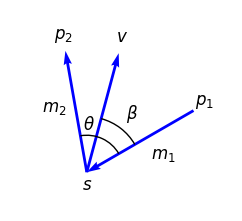
\includegraphics[width=0.5\textwidth]{circle}
        \caption{Diagram of $A^+$, $A^-$ and $B$}
    \end{wrapfigure}

    We can parametrize $v$ with the angle $\beta$ from $A^+$ (going toward $A^-$) and get to the following equation:
    \begin{equation}
        f(\epsilon) - f(0) = \epsilon \left[ (M-m)^\alpha - m^\alpha \cos\beta - M^\alpha (\cos\theta\cos\beta - \sin\theta\sin\beta) \right] + o(\epsilon)
    \end{equation}

    To prove that $\theta$ is not optimal we can either have $\exists \beta$ such that the above expression is negative or
    that $g(\beta) \ge 0$ for all $\beta$.

    Now we want to fix $\theta, M, m$ and study the minimum of this function:
    \begin{equation}
    (M-m)
        ^\alpha - m^\alpha \cos\beta - M^\alpha (\cos\theta\cos\beta - \sin\theta\sin\beta)
    \end{equation}

    Calling $t = \cos(\beta)$ we get the following equations needs to have a solution for $\beta$:
    \begin{equation}
    (M-m)
        ^{\alpha} + \cos\beta(-m^\alpha-M^\alpha t) + \sin\beta(M^\alpha \sqrt{1-t^2}) = 0
    \end{equation}

    Having a value of $\beta$ such that the above equation evaluates to 0 is not enough, we should also check if on one side there is
    a minimum.
    We also know there is a $\beta$ such that the value is negative (take beta outside of span of $A^+, A^-$ contradicting the convex
    hull property of the optimal solution). This implies that in case of non-optimal $\theta$ this function needs to pass
    through 0.


    By solving this equation (todo check condition $c^2 \le a^2 + b^2$) we get the condition:
    \begin{equation}
        t \ge \frac{(M-m)^{2\alpha} - M^{2\alpha} - m^{2\alpha}}{2m^\alpha M^\alpha}
    \end{equation}
    Which is almost the same as lemma 12.2. There are some signs which are different so maybe I should check the computation but the
    assumptions are also slightly different (in particular one of the flows is in the other direction, which explains the $M-m$ instead
    of $M+m$).

    General observation:
    this new bound can be used on every Steiner point, but we should be careful because due to degeneracy those points
    can also be in the support of the distribution.

    \subsection{Recap}
    We have two conditions, depending on the direction of the flows.
    If both flows are going in the same direction we have:
    \begin{equation}
        \cos(\theta) \le \frac{(m_1 + m_2) ^ {2\alpha} - m_1^{2\alpha} - m_2^{2\alpha}}{2m_1^\alpha m_2^\alpha}
        \label{eq:bound1}
    \end{equation}

    If one flow is going in the opposite direction we have:
    \begin{equation}
        \cos(\theta) \le \frac{(m_1 - m_2) ^ {2\alpha} - m_1^{2\alpha} - m_2^{2\alpha}}{2m_1^\alpha m_2^\alpha}
        \label{eq:bound2}
    \end{equation}

    We are just left to compute the maximum possible given the constraint that $m_1, m_2$ need to be a combination of the masses
    of the specific instance.

    \subsection{Solving the maximization problem}

    For the first case, we have two different behaviorurs depending on the value of $\alpha$:
    \begin{itemize}
        \item If $\alpha \le 1/2$ we have that the function is decreasing in $m_1$ for fixed $m_2$. Therefore the maximum is achieved when $m_1$ is the smallest and $m_2 = 1 - m_1$ (assuming the sum of the masses is 1).
        \item If $\alpha > 1/2$ we have that the function is increasing in $m_1$ for fixed $m_2$ and $m_1 \le m_2$. The maximum is achieved at $m_1 = m_2$ and we should aim to solve a closest subset sum problem.
    \end{itemize}

    The first case is easy, the second appears to be NP complete. In practice by the pigeonhole principle we have an upper bound on the distance of
    $1/n$ if there are n masses. Combining with the flatness of the function around $m_1 = m_2$ it might not be worth solving the problem exactly.
    We need a lower bound on the distance (rather than an upper bound) so it could be more difficult to obtain one, but if the upper bound is very close
    to the theoretical best (which is 0) we might just use the known sup $2^{2\alpha-1}-1$.

    It also seems that we could put a tolerance, as all values close to 0 give a very similar bound. (Maybe
    computing the second or third derivative around $m_1=m_2$ w.r.t. $m_1-m_2$ will give us a quantitative measure of).
    \\
    For the second case, we know this bound will be tighter than the first. We cannot know in advance the kind of angle we will encounter
    so we should just take the maximum among the two. This function exhibits a similar behaviour neverthless and we can refer to the
    graphs in the jupyter notebook.

    \subsection{From angle to degree}

    We know from \cite{coso sui cap sferici} that we can fit at most $C(\theta/2)$ arcs with distance among them at least $\beta$ where the expression for $C(\cdot)$
    is given by:
    \begin{enumerate}
        \item[(i)] \( C(\beta) = 1 \text{ for } \frac{1}{2}\pi < \beta \leq \pi; \)
        \item[(ii)] \( C(\beta) = \left\lfloor \frac{2 \sin^2 \beta}{2 \sin^2 \beta - 1} \right\rfloor \text{ for } \frac{1}{4}\pi + \frac{1}{2} \sin^{-1} \frac{1}{N} \leq \beta \leq \frac{1}{2}\pi; \)
        \item[(iii)] \( C(\beta) = N + 1 \text{ for } \frac{1}{4}\pi < \beta \leq \frac{1}{4}\pi + \frac{1}{2} \sin^{-1} \frac{1}{N}; \)
        \item[(iv)] \( C\left(\frac{1}{4}\pi\right) = 2N. \)
    \end{enumerate}

    If $0 < \beta < \frac{1}{4}\pi$ and $\gamma = \sin^{-1}\left(\frac{\sqrt{2} \sin \beta}{2}\right)$, then
    \begin{equation}
        C(\beta) \leq \frac{\pi \Gamma\left(\frac{N-1}{2}\right) \sin \gamma \tan \gamma}{2 \Gamma\left(\frac{N}{2}\right) \int_0^{\gamma} (\sin \phi)^{N-2} (\cos \phi - \cos \gamma) \, d\phi} = C^*(\beta)
    \end{equation}

    Further, for large $N$
    \begin{equation}
        C^*(\beta) \sim \frac{\frac{1}{2}\pi N^3 \cos 2\beta}{(\frac{\sqrt{2} \sin \beta}{2})^{N-1}}
    \end{equation}

    Provided that $\sec 2\beta = o(N)$.


    Therefore, if we have a bound on the angle $\theta$ (given by the max of (\ref{eq:bound1}) and (\ref{eq:bound2})) the degree of the Steiner points is given by:
    \begin{equation}
        deg(\beta, N) \leq C(\theta/2)
    \end{equation}

\end{document}
